\documentclass[a4paper]{article}

%=========================================
% Packages
%=========================================
\usepackage{mathtools}
\usepackage{amsfonts}
\usepackage{amsmath}
\usepackage{amssymb}
\usepackage{amsthm}
\usepackage[a4paper, total={6in, 8in}, margin=1in]{geometry}
\usepackage[utf8]{inputenc}
\usepackage{fancyhdr}
\usepackage[utf8]{inputenc}
\usepackage{graphicx}
\usepackage{physics}
\usepackage[listings]{tcolorbox}
\usepackage{hyperref}
\usepackage{tikz-cd}
\usepackage{adjustbox}
\usepackage{enumitem}
\usepackage[font=small,labelfont=bf]{caption}
\usepackage{subcaption}
\usepackage{wrapfig}
\usepackage{makecell}



\raggedright

\usetikzlibrary{arrows.meta}

\DeclarePairedDelimiter\ceil{\lceil}{\rceil}
\DeclarePairedDelimiter\floor{\lfloor}{\rfloor}

%=========================================
% Fonts
%=========================================
\usepackage{tgpagella}
\usepackage[T1]{fontenc}


%=========================================
% Custom Math Operators
%=========================================
\DeclareMathOperator{\adj}{adj}
\DeclareMathOperator{\im}{im}
\DeclareMathOperator{\nullity}{nullity}
\DeclareMathOperator{\sign}{sign}
\DeclareMathOperator{\dom}{dom}
\DeclareMathOperator{\lcm}{lcm}
\DeclareMathOperator{\ran}{ran}
\DeclareMathOperator{\ext}{Ext}
\DeclareMathOperator{\dist}{dist}
\DeclareMathOperator{\diam}{diam}
\DeclareMathOperator{\aut}{Aut}
\DeclareMathOperator{\inn}{Inn}
\DeclareMathOperator{\syl}{Syl}
\DeclareMathOperator{\edo}{End}
\DeclareMathOperator{\cov}{Cov}
\DeclareMathOperator{\vari}{Var}
\DeclareMathOperator{\cha}{char}
\DeclareMathOperator{\Span}{span}
\DeclareMathOperator{\ord}{ord}
\DeclareMathOperator{\res}{res}
\DeclareMathOperator{\Hom}{Hom}
\DeclareMathOperator{\Mor}{Mor}
\DeclareMathOperator{\coker}{coker}
\DeclareMathOperator{\Obj}{Obj}
\DeclareMathOperator{\id}{id}
\DeclareMathOperator{\GL}{GL}
\DeclareMathOperator*{\colim}{colim}

%=========================================
% Custom Commands (Shortcuts)
%=========================================
\newcommand{\CP}{\mathbb{CP}}
\newcommand{\GG}{\mathbb{G}}
\newcommand{\F}{\mathbb{F}}
\newcommand{\N}{\mathbb{N}}
\newcommand{\Q}{\mathbb{Q}}
\newcommand{\R}{\mathbb{R}}
\newcommand{\C}{\mathbb{C}}
\newcommand{\E}{\mathbb{E}}
\newcommand{\Prj}{\mathbb{P}}
\newcommand{\RP}{\mathbb{RP}}
\newcommand{\T}{\mathbb{T}}
\newcommand{\Z}{\mathbb{Z}}
\newcommand{\A}{\mathbb{A}}
\renewcommand{\H}{\mathbb{H}}
\newcommand{\K}{\mathbb{K}}

\newcommand{\mA}{\mathcal{A}}
\newcommand{\mB}{\mathcal{B}}
\newcommand{\mC}{\mathcal{C}}
\newcommand{\mD}{\mathcal{D}}
\newcommand{\mE}{\mathcal{E}}
\newcommand{\mF}{\mathcal{F}}
\newcommand{\mG}{\mathcal{G}}
\newcommand{\mH}{\mathcal{H}}
\newcommand{\mI}{\mathcal{I}}
\newcommand{\mJ}{\mathcal{J}}
\newcommand{\mK}{\mathcal{K}}
\newcommand{\mL}{\mathcal{L}}
\newcommand{\mM}{\mathcal{M}}
\newcommand{\mO}{\mathcal{O}}
\newcommand{\mP}{\mathcal{P}}
\newcommand{\mS}{\mathcal{S}}
\newcommand{\mT}{\mathcal{T}}
\newcommand{\mV}{\mathcal{V}}
\newcommand{\mW}{\mathcal{W}}

%=========================================
% Colours!!!
%=========================================
\definecolor{LightBlue}{HTML}{2D64A6}
\definecolor{ForestGreen}{HTML}{4BA150}
\definecolor{DarkBlue}{HTML}{000080}
\definecolor{LightPurple}{HTML}{cc99ff}
\definecolor{LightOrange}{HTML}{ffc34d}
\definecolor{Buff}{HTML}{DDAE7E}
\definecolor{Sunset}{HTML}{F2C57C}
\definecolor{Wenge}{HTML}{584B53}
\definecolor{Coolgray}{HTML}{9098CB}
\definecolor{Lavender}{HTML}{D6E3F8}
\definecolor{Glaucous}{HTML}{828BC4}
\definecolor{Mauve}{HTML}{C7A8F0}
\definecolor{Darkred}{HTML}{880808}
\definecolor{Beaver}{HTML}{9A8873}
\definecolor{UltraViolet}{HTML}{52489C}



%=========================================
% Theorem Environment
%=========================================
\tcbuselibrary{listings, theorems, breakable, skins}

\newtcbtheorem[number within = subsection]{thm}{Theorem}%
{	colback=Buff!3, 
	colframe=Buff, 
	fonttitle=\bfseries, 
	breakable, 
	enhanced jigsaw, 
	halign=left
}{thm}

\newtcbtheorem[number within=subsection, use counter from=thm]{defn}{Definition}%
{  colback=cyan!1,
    colframe=cyan!50!black,
	fonttitle=\bfseries, breakable, 
	enhanced jigsaw, 
	halign=left
}{defn}

\newtcbtheorem[number within=subsection, use counter from=thm]{axm}{Axiom}%
{	colback=red!5, 
	colframe=Darkred, 
	fonttitle=\bfseries, 
	breakable, 
	enhanced jigsaw, 
	halign=left
}{axm}

\newtcbtheorem[number within=subsection, use counter from=thm]{prp}{Proposition}%
{	colback=LightBlue!3, 
	colframe=Glaucous, 
	fonttitle=\bfseries, 
	breakable, 
	enhanced jigsaw, 
	halign=left
}{prp}

\newtcbtheorem[number within=subsection, use counter from=thm]{lmm}{Lemma}%
{	colback=LightBlue!3, 
	colframe=LightBlue!60, 
	fonttitle=\bfseries, 
	breakable, 
	enhanced jigsaw, 
	halign=left
}{lmm}

\newtcbtheorem[number within=subsection, use counter from=thm]{crl}{Corollary}%
{	colback=LightBlue!3, 
	colframe=LightBlue!60, 
	fonttitle=\bfseries, 
	breakable, 
	enhanced jigsaw, 
	halign=left
}{crl}

\newtcbtheorem[number within=subsection, use counter from=thm]{eg}{Example}%
{	colback=Beaver!5, 
	colframe=Beaver, 
	fonttitle=\bfseries, 
	breakable, 
	enhanced jigsaw, 
	halign=left
}{eg}

\newtcbtheorem[number within=subsection, use counter from=thm]{ex}{Exercise}%
{	colback=Beaver!5, 
	colframe=Beaver, 
	fonttitle=\bfseries, 
	breakable, 
	enhanced jigsaw, 
	halign=left
}{ex}

\newtcbtheorem[number within=subsection, use counter from=thm]{alg}{Algorithm}%
{	colback=UltraViolet!5, 
	colframe=UltraViolet, 
	fonttitle=\bfseries, 
	breakable, 
	enhanced jigsaw, 
	halign=left
}{alg}




%=========================================
% Hyperlinks
%=========================================
\hypersetup{
    colorlinks=true, %set true if you want colored links
    linktoc=all,     %set to all if you want both sections and subsections linked
    linkcolor=DarkBlue,  %choose some color if you want links to stand out
}


\pagestyle{fancy}
\fancyhf{}
\rhead{Labix}
\lhead{Algebraic Topology 4}
\rfoot{\thepage}

\title{Algebraic Topology 4}

\author{Labix}

\date{\today}
\begin{document}
\maketitle
\begin{abstract}
\end{abstract}
~\\~\\
References: 
\begin{itemize}
\item Notes on Algebraic Topology by Oscar Randal-Williams: \\
The first chapter gives a complete treatment of the first three sections of these notes, as well as providing the importance of fibrations on the higher homotopy groups. These notes are highly recommended to understanding the first three sections. 

\item Algebraic Topology by Allen Hatcher: \\
A more or less complete dictionary on all topics of these notes. However it is prone to the same problem in the sense that Hatcher's book is rather terse and definitions and parts of some theorems are scattered throughout the paragraphs rather than having a complete statement for reference. Nevertheless it is still the standard reference of the notes, albeit organized in a slightly different way. 

\item A non-visual proof that higher homotopy groups are abelian by Shintaro Fushida-Hardy: \\
This short piece of article proves that the higher homotopy groups are abelian in a purely algebraic way. Most geometric visualization of such a proof has the same underlying idea as the algebraic method. 
\end{itemize}

\pagebreak
\tableofcontents

\pagebreak
\section{The Fundamental Groupoid and Covering Space Theory}
\subsection{The Fundamental Groupoid}
\begin{defn}{The Fundamental Groupoid}{} Let $X$ be a space. Define the fundamental groupoid $\Pi_1X$ of $X$ to be the category with the following data. 
\begin{itemize}
\item The objects are the points of $X$. 
\item Let $x,y\in X$. The morphisms of $\Pi_1X$ are given by $$\Hom_{\Pi_1X}(x,y)=\{\gamma:I\to X\;|\;\gamma(0)=x\text{ and }\gamma(1)=y\text{ is a path }\}/\sim$$ where we say that two paths are equivalent if they are homotopic. 
\item Composition is defined by the concatenation of paths. 
\end{itemize}
\end{defn}

We have seen in Algebraic Topology 1 that composition of homotopy classes of paths are well defined. 

\begin{lmm}{}{} Let $X$ be a space. Then $\Pi_1X$ is a groupoid. \tcbline
\begin{proof}
Every path in $X$ has an inverse that lies in $\Pi_1X$ given by reversing traversal of the path. 
\end{proof}
\end{lmm}

\begin{lmm}{}{} Let $X$ be a space and $x_0\in X$. Then there is a group isomorphism $$\Hom_{\Pi_1X}(x_0,x_0)\cong\pi_1(X,x_0)$$
\end{lmm}

\begin{prp}{}{} Let $f:X\to Y$ be a continuous map. Then $f$ induces a functor $\Pi_1f:\Pi_1X\to\Pi_1Y$ defined by $$\Pi_1f([\alpha])=[f\circ\alpha]$$ on morphisms. \tcbline
\begin{proof}
Direct from Algebraic Topology 1 due to the above group isomorphism. We have also seen that it is functorial in Algebraic Topology 1. 
\end{proof}
\end{prp}

\begin{thm}{}{} The fundamental groupoid defines a functor $\Pi_1:\bold{Top}\to\bold{Grps}$ from the category of spaces to the category of groupoids with the following data. 
\begin{itemize}
\item $\Pi_1$ sends each space $X$ to $\Pi_1X$
\item $\Pi_1$ sends each continuous map $f:X\to Y$ to the functor $\Pi_1f$
\end{itemize}
\end{thm}

\subsection{The Seifert-Van Kampen Theorem on Fundamental Groupoids}
\begin{defn}{The Fundamental Groupoid of Subspaces}{} Let $X$ be a space and $A\subseteq X$ a subspace. Define $\Pi_1X[A]$ to be the full subcategory of $\Pi_1X$ where the objects are $A$. Explicitly, $\Pi_1X[A]$ consists of the following data. 
\begin{itemize}
\item The objects of $\Pi_1X[A]$ are the points of $A$. 
\item The morphisms are given by $$\Hom_{\Pi_1X[A]}(x,y)=\Hom_{\Pi_1X}(x,y)$$ for any $x,y\in X$. 
\item Composition is inherited from $\Pi_1X$. 
\end{itemize}
\end{defn}

\begin{lmm}{}{} Let $X$ be a space and $A\subseteq X$ a subspace of $X$ such that every path component of $X$ contains a point of $A$. Then the inclusion $$\Pi_1X[A]\to\Pi_1X$$ of groupoids is an equivalence of categories. \tcbline
\begin{proof}
The inclusion is already fully faithful since $\Pi_1X[A]$ is a full subcategory. Now let $x\in X$. Let $a\in A$ lie in the same path component as $x$. Let $\alpha:I\to X$ be a path from $x$ to $a$. Then the morphism $[\alpha]:x\to a$ of $\Pi_1X$ is an isomorphism since $\Pi_1X$ is a groupoid. Thus we conclude. 
\end{proof}
\end{lmm}

\begin{crl}{}{} Let $X$ be a space. Then there is an equivalence of categories $$\coprod_{[x_0]\in\pi_0(X)}B\pi_0(X,x_0)\cong\Pi_1X$$ \tcbline
\begin{proof}
This is done by choosing $A$ to contain exactly one point of each path component, and then by applying the isomorphism $$\Pi_1X[x_0]=B\text{Aut}_{\Pi_1X}(x_0)=B\pi_1(X,x_0)$$ and the above lemma. 
\end{proof}
\end{crl}

If $X$ is path connected, then this shows that any choice of base point $x_0\in X$ gives an equivalence of categories $$B\pi_0(X,x_0)\cong\Pi_1X$$ This translates roughly to the standard fact in Algebraic Topology that the fundamental group of a path connected space for any two base points are isomorphic. Indeed in the equivalence of categories exhibited, the former depends on the base point while the latter does not. \\~\\

We need a lemma. 

\begin{lmm}{}{} Let $\mJ$ and $\mC$ be categories and let $\mJ$ be the following category \\~\\
\adjustbox{scale=1.0,center}{\begin{tikzcd}
	0 & 1 \\
	2 & 3
	\arrow[from=1-1, to=1-2]
	\arrow[from=1-1, to=2-1]
	\arrow["i", from=1-2, to=2-2]
	\arrow["j"', from=2-1, to=2-2]
\end{tikzcd}} \\~\\
such that $Y:\mJ\to\mC$ is a pushout diagram. If $p:Y\Rightarrow X$ is a natural transformations such that $p$ is a retraction, then $X:\mJ\to\mC$ is also a pushout diagram. \tcbline
\begin{proof}
Consider the following diagram: \\~\\
\adjustbox{scale=1.0,center}{\begin{tikzcd}
	{X_0} && {X_1} \\
	& {Y_0} && {Y_1} \\
	{X_2} && {X_3} \\
	& {Y_2} && {Y_3} 
	\arrow[from=1-1, to=1-3]
	\arrow["{s_0}"', shift right, from=1-1, to=2-2]
	\arrow[from=1-1, to=3-1]
	\arrow["{s_1}"', shift right, from=1-3, to=2-4]
	\arrow["{X(i)}"'{pos=0.3}, from=1-3, to=3-3]
	\arrow["{p_0}"', shift right, from=2-2, to=1-1]
	\arrow["{p_1}"', shift right, from=2-4, to=1-3]
	\arrow["{Y(i)}"', from=2-4, to=4-4]
	\arrow["{X(j)}"{pos=0.3}, from=3-1, to=3-3]
	\arrow["{s_2}"', shift right, from=3-1, to=4-2]
	\arrow["{s_3}"', shift right, from=3-3, to=4-4]
	\arrow["{p_2}"', shift right, from=4-2, to=3-1]
	\arrow["{Y(j)}"', from=4-2, to=4-4]
	\arrow["{p_3}"', shift right, from=4-4, to=3-3]
	\arrow[from=2-2, to=2-4, crossing over]
	\arrow[from=2-2, to=4-2, crossing over]
\end{tikzcd}} \\~\\
This diagram is commutative by the following reasons. 
\begin{itemize}
\item The front and back face of the square commutes since $X$ and $Y$ are functors and functors preserve commutative diagrams. 
\item The rest of the faces of the square commutes by the natural transformations $p$ and $s$. 
\end{itemize}

Let $Z\in\mC$ such that there are maps $\lambda_1:X_1\to Z$ and $\lambda_2:X_2\to Z$ for which the maps $$X_0\to X_1\overset{\lambda_1}{\longrightarrow} Z\;\;\;\;\text{ and }\;\;\;\;X_0\to X_2\overset{\lambda_2}{\longrightarrow}Z$$ are equal. Then in particular the two maps $$Y_0\to X_0\to X_1\overset{\lambda_1}{\longrightarrow} Z\;\;\;\;\text{ and }\;\;\;\;Y_0\to X_0\to X_2\overset{\lambda_2}{\longrightarrow}Z$$ are equal. By commutativity of the cube, the two maps $$Y_0\to Y_1\overset{p_1}{\longrightarrow} X_1\overset{\lambda_1}{\longrightarrow} Z\;\;\;\;\text{ and }\;\;\;\;Y_0\to Y_2\overset{p_2}{\longrightarrow} X_2\overset{\lambda_2}{\longrightarrow}Z$$ are equal. By the universal property of $Y_3$ as a pushout diagram, there exists a unique map $Y_3\to Z$. such that the following diagram commutes: \\~\\
\adjustbox{scale=1.0,center}{\begin{tikzcd}
	{X_0} && {X_1} \\
	& {Y_0} && {Y_1} \\
	{X_2} && {X_3} \\
	& {Y_2} && {Y_3} \\
	&&&& Z
	\arrow[from=1-1, to=1-3]
	\arrow["{s_0}"', shift right, from=1-1, to=2-2]
	\arrow[from=1-1, to=3-1]
	\arrow["{s_1}"', shift right, from=1-3, to=2-4]
	\arrow["{X(i)}"'{pos=0.3}, from=1-3, to=3-3]
	\arrow["{p_0}"', shift right, from=2-2, to=1-1]
	\arrow["{p_1}"', shift right, from=2-4, to=1-3]
	\arrow["{Y(i)}"', from=2-4, to=4-4]
	\arrow["{\lambda_1}", from=1-3, to=5-5, bend left = 60]
	\arrow["{X(j)}"{pos=0.3}, from=3-1, to=3-3]
	\arrow["{s_2}"', shift right, from=3-1, to=4-2]
	\arrow["{s_3}"', shift right, from=3-3, to=4-4]
	\arrow["{p_2}"', shift right, from=4-2, to=3-1]
	\arrow["{Y(j)}"', from=4-2, to=4-4]
	\arrow["{\lambda_2}"', from=3-1, to=5-5, bend right = 60]
	\arrow["{p_3}"', shift right, from=4-4, to=3-3]
	\arrow["{\exists!}"{description}, dashed, from=4-4, to=5-5]
	\arrow[from=2-2, to=2-4, crossing over]
	\arrow[from=2-2, to=4-2, crossing over]
\end{tikzcd}} \\~\\
Since the retraction of a map is unique, $s$ is unique. Also the map $Y_3\to Z$ is unique by definition of pushout diagram. Hence there is a unique map $X_3\to Y_3\to Z$ so that $X$ is a pushout diagram. 
\end{proof}
\end{lmm}

\begin{thm}{The Seifert-Van Kampen Theorem on Fundamental Groupoids}{} Let $X$ be a space and $U,V\subseteq X$ an open cover of $X$. Let $A\subseteq X$ be a subspace such that every path connected component of $U,V,X$ contains a point in $A$. Then the inclusions $$\Pi_1(U\cap V)[U\cap V\cap A]\to\Pi_1U[U\cap A]\;\;\;\;\text{ and }\;\;\;\Pi_1(U\cap V)[U\cap V\cap A]\to\Pi_1V[V\cap A]$$ give a pushout diagram to $\Pi_1X[A]$. This means that the following diagram is a pushout: \\~\\
\adjustbox{scale=1.0,center}{\begin{tikzcd}
	{\Pi_1(U\cap V)[U\cap V\cap A]} & {\Pi_1U[U\cap A]} \\
	{\Pi_1V[V\cap A]} & {\Pi_1X[A]}
	\arrow[from=1-1, to=1-2]
	\arrow[from=1-1, to=2-1]
	\arrow[from=1-2, to=2-2]
	\arrow[from=2-1, to=2-2]
\end{tikzcd}} \\~\\
where each arrow is an inclusions. 
\tcbline
\begin{proof}
First assume that $X=A$. We want to show that for any groupoid $\mG\in\bold{Grp}$ with maps $\Pi_1U,\Pi_1V\to\mG$, there exists a unique map $\Pi_1X\to\mG$ such that the following diagram commutes: \\~\\
\adjustbox{scale=1.0,center}{\begin{tikzcd}
	{\Pi_1(U\cap V)} & {\Pi_1U} \\
	{\Pi_1V} & {\Pi_1X} \\
	&& \mG
	\arrow[from=1-1, to=1-2]
	\arrow[from=1-1, to=2-1]
	\arrow[from=1-2, to=2-2]
	\arrow[from=1-2, to=3-3, bend left = 20, "f"]
	\arrow[from=2-1, to=2-2]
	\arrow[from=2-1, to=3-3, bend right = 20, "g"]
	\arrow[from=2-2, to=3-3, dashed, "\exists!u"]
\end{tikzcd}}\\~\\
Define the functor $u:\Pi_1X\to\mG$ as follows. For each $x\in\Pi_1X$, define $$u(x)=\begin{cases}
f(x) & \text{ if }x\in U\\
g(x) & \text{ if }x\in V
\end{cases}$$ This is well defined on $U\cap V$ since the outer square of the above diagram commutes. Depending on the path in $X$, there will be different constructions. Let $[\alpha]$ be a morphism in $\Pi_1X$. If $\alpha:I\to X$ has image in $U$, then define $u([\alpha])=f([\alpha])$. Similarly, define $u([\alpha])=g([\alpha])$ if $\alpha$ has image in $V$. \\~\\

Otherwise, by the Lebesgue covering theorem, there is a finite sequence $0=a_0<a_1<\cdots<a_n=1$ such that $\alpha([a_i,a_{i+1}])\subseteq U$ or $V$. Define $\alpha_i=\alpha\;|\;_{a_i,a_{i+1}}$. It is easy to see that 
\begin{align*}
[\alpha]&=[\alpha\;|\;_{0,a_1}]\cdot[\alpha\;|\;_{a_1,a_2}]\cdots[\alpha\;|\;_{a_{n-1},1}]\tag{Viewed as paths}\\
&=[\alpha_{n-1}]\circ\cdots[\alpha_1]\circ[\alpha_0]\tag{Viewed as morphisms in $\Pi_1X$}
\end{align*} Then we can define $u(\alpha)$ as $$u([\alpha])=u([\alpha_{n-1}])\circ u(\cdots[\alpha_1])\circ u([\alpha_0])$$ where we have that $$u([\alpha_i])=\begin{cases}
f([\alpha_i]) & \text{ if }\im(\alpha_i)\subseteq U\\
g([\alpha_i]) & \text{ if }\im(\alpha_i)\subseteq V
\end{cases}$$ If $u$ exists, then $u$ must take the above form. Thus we have shown uniqueness. \\~\\

For existence, we have to show that above construction of $u$ is well defined. Let $\alpha,\beta$ be paths in $X$ from $x$ to $y$ that are homotopic via the map $H:I\times I\to X$. We want to show that $u([\alpha])=u([\beta])$. By the Lebesgue covering theorem, there is a grid in $I\times I$ where the $x$-axis is subdivided into $0=a_0<a_1<\cdots<a_n=1$ and the $y$-axis is subdivided into $0=c_0<c_1<\cdots<c_k=1$.  such that $H$ sends each rectangle with vertices $\{a_i,a_{i+1},c_j,c_{j+1}\}$ to either $U$ or $V$. Let $h^j=H(-,c_j):I\to X$ so that $h^0=\alpha$ and $h^k=\beta$. Define $$\delta_i=H(\alpha_i,-)\;|\;_{[c_j,c_{j+1}]}:I\to X$$ which are paths from $(a_i,c_j)$ to $(a_i,c_{j+1})$ in $I\times I$. Also define $h_i^j=h^j\;|\;_{[\alpha_i,\alpha_{i+1}]}$. Now we have the following which lies entirely in $X$: 

\begin{center}
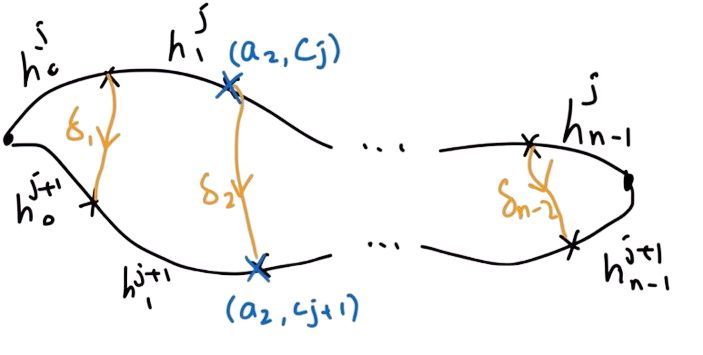
\includegraphics[scale = 0.3]{Image 1}
\end{center}

Now we have that 
\begin{align*}
u([h^j])&=u([h_{n-1}^j])\circ\cdots\circ u([h_0^j])\\
&=u([h_{n-1}^{j+1}\circ\delta_{n-2}])\circ u([\overline{\delta_{n-2}}\circ h_{n-2}^{j+1}\circ\delta_{n-3}])\circ\cdots\circ u([\overline{\delta_1}\circ h_0^{j+1}])\\
&=u([h_{n-1}^{j+1}])\circ\cdots\circ u([h_0^{j+1}])\\
&=u([h^{j+1}])
\end{align*}
By induction, we conclude that $$u([\alpha])=u([h^0])=u([h^1])=\dots=u([h^k])=u([\beta])$$~\\

Now suppose that $A\subseteq X$. By the above lemma, it is sufficient to show that the square for $A$ is a retract of the square for $X$. Let $x\in U\cap V$ and $a_x\in A\cap U\cap V$ lying in the same path component as $x$. Choose a path $\alpha_x:I\to X$ from $a_x$ to $x$ with $\alpha_x$ being constant if $x\in A$. Do a similar choice for $x\in U\setminus(U\cap V)$ and $x\in V\setminus(U\cap V)$. Define $p_{U\cap V}:\Pi_1(U\cap V)\to\Pi_1(U\cap V)[U\cap V\cap A]$ defined by $x\mapsto a_x$ on objects and $$[x\overset{\alpha}{\to} y]\mapsto\left(a_x\overset{[\alpha_x]}{\to}x\overset{[\alpha]}{\to}y\overset{[\alpha_y]}{\to}a_y\right)$$ and similarly for $p_U$ and $p_V$. This defines the natural transformation $p$ in lemma 5.3.4. We conclude by lemma 5.3.4. 
\end{proof}
\end{thm}

Take $A=\{x_0\}$ be a single point in $U\cap V$. Then this theorem shows that there is a pushout diagram \\~\\
\adjustbox{scale=1.0,center}{\begin{tikzcd}
	{\pi_1(U\cap V,x_0)} & {\pi_1(U,x_0)} \\
	{\pi_1(V,x_0)} & {\pi_1(X,x_0)}
	\arrow[from=1-1, to=1-2]
	\arrow[from=1-1, to=2-1]
	\arrow[from=1-2, to=2-2]
	\arrow[from=2-1, to=2-2]
\end{tikzcd}}\\~\\
in $\bold{Grp}$, provided that $A$ contains every path connected component of $U,V,X$. But $A$ is just one point so the condition becomes that $U,V,X$ and $U\cap V$ being path connected. Hence we recover the usual Seifert-Van Kampen theorem in Algebraic Topology 1. 

\subsection{Categorical Covering Space Theory}
We end the section with a categorical approach of the Galois correspondence between covering spaces and the fundamental group. 

\begin{defn}{Category of Covering Spaces of a Space}{} Let $X$ be a space. Define the category $\text{Cov}(X)$ of covering spaces of $X$ by the following. 
\begin{itemize}
\item The objects are the covering spaces $p:\tilde{X}\to X$ of $X$
\item For two covering spaces $p_1:\tilde{X}_1\to X$ and $p_2:\tilde{X}_2\to X$ of $X$, a morphism is a map $q:\tilde{X}_1\to\tilde{X}_2$ such that following diagram commutes: \\~\\
\adjustbox{scale=1.0,center}{\begin{tikzcd}
\tilde{X}_1\arrow[rr, "q"]\arrow[rdd, "p_1"'] && \tilde{X}_2\arrow[ldd, "p_2"] \\
&&\\
& X &
\end{tikzcd}}
\item Composition is given by the composition of functions. 
\end{itemize}
\end{defn}

Recall the category $G\text{-Set}$ of $G$-sets for a group $G$ to consist of the following data. 
\begin{itemize}
\item The objects are sets which have a group action $G$. 
\item For two $G$-sets $X$ and $Y$, a morphism is a $G$-equivariant function $f:X\to Y$. This means that $$f(g\cdot x)=g\cdot f(x)$$ for all $g\in G$ and $x\in X$. 
\item Composition is given by the composition of functions. 
\end{itemize}

\begin{thm}{}{} Let $X$ be a connected and locally simply connected space. Let $x_0\in X$. The the functor $F:\text{Cov}(X)\to\pi_1(X,x_0)\text{-Set}$ defined by $\left(p:\tilde{X}\to X\right)\mapsto p^{-1}(x_0)$ and $\left(q:\tilde{X}_1\to\tilde{X}_2\right)\mapsto q|_{p^{-1}(x_0)}$ gives an equivalence of categories $$\text{Cov}(X)\cong\pi_1(X,x_0)\text{-Set}$$
\end{thm}

\pagebreak
\section{Localizations of Spaces}
\subsection{T-Local Groups}
\begin{defn}{T-Local Groups}{} Let $G$ be a group and let $T$ be a set of prime. We say that $G$ is $T$-local if for all prime $p$ not in $T$, The $p$th power map $G\to G$ is a bijection. 
\end{defn}

\begin{lmm}{}{} Let $G$ be a group. Then for any prime $p$, the $p$th power map $G\to G$ is a group homomorphism. 
\end{lmm}

\begin{defn}{Localization on a Set of Prime}{} Let $T$ be a set of primes. Define the localization of $\Z$ at the set $T$ by $$\Z_T=(\Z\setminus T)^{-1}\Z$$
\end{defn}

\begin{prp}{}{} Let $G$ be abelian. Let $T$ be a set of primes. Then the following are equivalent. 
\begin{itemize}
\item $G$ is $T$-local
\item $G$ admits a unique structure of a $\Z_T$-module
\item For all prime $p$ not in $T$, $G\otimes\Z/p\Z=0$. 
\end{itemize}
\end{prp}

Recall that tensoring an abelian group $\Z/p\Z$ detects whether $G$ has torsion $\Z/p\Z$. If it is $0$ it means that $G$ contains no torsion groups of $p^n$ for all $n\in\N$. 

\begin{lmm}{}{} Let $A,B,C$ be abelian groups such that there is an exact sequence of the form \\~\\
\adjustbox{scale=1,center}{\begin{tikzcd}
	0 & A & B & C & 0
	\arrow[from=1-1, to=1-2]
	\arrow[from=1-2, to=1-3]
	\arrow[from=1-3, to=1-4]
	\arrow[from=1-4, to=1-5]
\end{tikzcd}}\\~\\
If two out of $A,B,C$ are $T$-local, then the third one is also $T$-local. 
\end{lmm}

TBA: Localization is an exact functor Ab to Mod $\Z_T$. 

\subsection{T-Local Spaces}
\begin{defn}{T-Equivalent Maps}{} Let $f:X\to Y$ be a map and let $T$ be a set of primes. We say that $f$ is $T$-equivalent if $$f_\ast:H_n(A;\Z_T)\to H_n(B;\Z_T)$$ is an isomorphism for all $n\in\N$. 
\end{defn}

\begin{defn}{T-Local Spaces}{} Let $X$ be space and let $T$ be a set of primes. We say that $X$ is a $T$-local space if for all $T$-equivalent maps $f:A\to B$, the induced map $$f^\ast:[B,X]\to[A,X]$$ is a bijection. 
\end{defn}

\begin{thm}{}{} Let $X$ be a space and let $T$ be a set of primes. Then the following conditions are equivalent for $X$. 
\begin{itemize}
\item $X$ is $T$-local
\item Each homotopy group $\pi_n(X)$ is $T$-local
\item Each homology group $H_n(X)$ is $T$-local
\end{itemize}
\end{thm}

\begin{prp}{}{} Let $A$ be an abelian group and let $T$ be a set of prime. Then $A$ is $T$-local if and only if $K(A,1)$ is $T$-local. 
\end{prp}

\begin{defn}{Localization of a Space}{} Let $X$ be a space and let $T$ be a set of primes. A localization of $X$ at $T$ is a $T$-local space $X_T$ together with a $T$-equivalent map $f:X\to X_T$ such that the following universal property is satisfied. For any map $g:X\to Z$ where $Z$ is a $T$-local space, there exists a map $h:X_T\to Z$ unique up to homotopy such that the following diagram commutes: \\~\\
\adjustbox{scale=1,center}{\begin{tikzcd}
	X & Z \\
	{X_T}
	\arrow["g", from=1-1, to=1-2]
	\arrow["f"', from=1-1, to=2-1]
	\arrow["{\exists h}"', dashed, from=2-1, to=1-2]
\end{tikzcd}}\\~\\
\end{defn}

To be added: functoriality of localization

\begin{thm}{}{} Every nilpotent space $X$ admits a localization at any set of primes $T$. 
\end{thm}

\pagebreak
\section{Completion of Spaces}








\end{document}
